\documentclass[twoside]{book}

% Packages required by doxygen
\usepackage{fixltx2e}
\usepackage{calc}
\usepackage{doxygen}
\usepackage[export]{adjustbox} % also loads graphicx
\usepackage{graphicx}
\usepackage[utf8]{inputenc}
\usepackage{makeidx}
\usepackage{multicol}
\usepackage{multirow}
\PassOptionsToPackage{warn}{textcomp}
\usepackage{textcomp}
\usepackage[nointegrals]{wasysym}
\usepackage[table]{xcolor}

% Font selection
\usepackage[T1]{fontenc}
\usepackage[scaled=.90]{helvet}
\usepackage{courier}
\usepackage{amssymb}
\usepackage{sectsty}
\renewcommand{\familydefault}{\sfdefault}
\allsectionsfont{%
  \fontseries{bc}\selectfont%
  \color{darkgray}%
}
\renewcommand{\DoxyLabelFont}{%
  \fontseries{bc}\selectfont%
  \color{darkgray}%
}
\newcommand{\+}{\discretionary{\mbox{\scriptsize$\hookleftarrow$}}{}{}}

% Page & text layout
\usepackage{geometry}
\geometry{%
  a4paper,%
  top=2.5cm,%
  bottom=2.5cm,%
  left=2.5cm,%
  right=2.5cm%
}
\tolerance=750
\hfuzz=15pt
\hbadness=750
\setlength{\emergencystretch}{15pt}
\setlength{\parindent}{0cm}
\setlength{\parskip}{0.2cm}
\makeatletter
\renewcommand{\paragraph}{%
  \@startsection{paragraph}{4}{0ex}{-1.0ex}{1.0ex}{%
    \normalfont\normalsize\bfseries\SS@parafont%
  }%
}
\renewcommand{\subparagraph}{%
  \@startsection{subparagraph}{5}{0ex}{-1.0ex}{1.0ex}{%
    \normalfont\normalsize\bfseries\SS@subparafont%
  }%
}
\makeatother

% Headers & footers
\usepackage{fancyhdr}
\pagestyle{fancyplain}
\fancyhead[LE]{\fancyplain{}{\bfseries\thepage}}
\fancyhead[CE]{\fancyplain{}{}}
\fancyhead[RE]{\fancyplain{}{\bfseries\leftmark}}
\fancyhead[LO]{\fancyplain{}{\bfseries\rightmark}}
\fancyhead[CO]{\fancyplain{}{}}
\fancyhead[RO]{\fancyplain{}{\bfseries\thepage}}
\fancyfoot[LE]{\fancyplain{}{}}
\fancyfoot[CE]{\fancyplain{}{}}
\fancyfoot[RE]{\fancyplain{}{\bfseries\scriptsize Generated on Sat Sep 26 2015 03\+:04\+:45 for Table Generator by Doxygen }}
\fancyfoot[LO]{\fancyplain{}{\bfseries\scriptsize Generated on Sat Sep 26 2015 03\+:04\+:45 for Table Generator by Doxygen }}
\fancyfoot[CO]{\fancyplain{}{}}
\fancyfoot[RO]{\fancyplain{}{}}
\renewcommand{\footrulewidth}{0.4pt}
\renewcommand{\chaptermark}[1]{%
  \markboth{#1}{}%
}
\renewcommand{\sectionmark}[1]{%
  \markright{\thesection\ #1}%
}

% Indices & bibliography
\usepackage{natbib}
\usepackage[titles]{tocloft}
\setcounter{tocdepth}{3}
\setcounter{secnumdepth}{5}
\makeindex

% Hyperlinks (required, but should be loaded last)
\usepackage{ifpdf}
\ifpdf
  \usepackage[pdftex,pagebackref=true]{hyperref}
\else
  \usepackage[ps2pdf,pagebackref=true]{hyperref}
\fi
\hypersetup{%
  colorlinks=true,%
  linkcolor=blue,%
  citecolor=blue,%
  unicode%
}

% Custom commands
\newcommand{\clearemptydoublepage}{%
  \newpage{\pagestyle{empty}\cleardoublepage}%
}


%===== C O N T E N T S =====

\begin{document}

% Titlepage & ToC
\hypersetup{pageanchor=false,
             bookmarks=true,
             bookmarksnumbered=true,
             pdfencoding=unicode
            }
\pagenumbering{roman}
\begin{titlepage}
\vspace*{7cm}
\begin{center}%
{\Large Table Generator }\\
\vspace*{1cm}
{\large Generated by Doxygen 1.8.9.1}\\
\vspace*{0.5cm}
{\small Sat Sep 26 2015 03:04:45}\\
\end{center}
\end{titlepage}
\clearemptydoublepage
\tableofcontents
\clearemptydoublepage
\pagenumbering{arabic}
\hypersetup{pageanchor=true}

%--- Begin generated contents ---
\chapter{Table Generator}
\label{md_README}
\hypertarget{md_README}{}
Project to generate A\+S\+C\+I\+I based tables from user data

\subsubsection*{Introduction}

\hyperlink{classTable}{Table} Generator reads a file having delimeted table elements and creates a formatted table.

\subsection*{Class Diagram}

\subsubsection*{Usage}

\subsubsection*{Examples}

Input\+:

No. Professor Course Name Course Number 1 Dr. Heber Design and Analysis of Algorithms C\+S\+C505 2 Dr. Dutta Internet Protocols C\+S\+C573 3 Dr. Perros Networking Services C\+S\+C576

Output from \hyperlink{classFairFormatter}{Fair\+Formatter}\+:

+-\/-\/---+-\/-\/-\/-\/-\/-\/-\/-\/-\/---+-\/-\/-\/-\/-\/-\/-\/-\/-\/-\/-\/-\/-\/-\/-\/-\/-\/-\/-\/-\/-\/-\/-\/-\/-\/-\/-\/-\/-\/-\/-\/-\/---+-\/-\/-\/-\/-\/-\/-\/-\/-\/-\/-\/-\/---+ $\vert$\+No. $\vert$\+Professor $\vert$\+Course Name $\vert$\+Course Number $\vert$ +-\/-\/---+-\/-\/-\/-\/-\/-\/-\/-\/-\/---+-\/-\/-\/-\/-\/-\/-\/-\/-\/-\/-\/-\/-\/-\/-\/-\/-\/-\/-\/-\/-\/-\/-\/-\/-\/-\/-\/-\/-\/-\/-\/-\/---+-\/-\/-\/-\/-\/-\/-\/-\/-\/-\/-\/-\/---+ $\vert$1 $\vert$\+Dr. Heber $\vert$\+Design and Analysis of Algorithms $\vert$\+C\+S\+C505 $\vert$ +-\/-\/---+-\/-\/-\/-\/-\/-\/-\/-\/-\/---+-\/-\/-\/-\/-\/-\/-\/-\/-\/-\/-\/-\/-\/-\/-\/-\/-\/-\/-\/-\/-\/-\/-\/-\/-\/-\/-\/-\/-\/-\/-\/-\/---+-\/-\/-\/-\/-\/-\/-\/-\/-\/-\/-\/-\/---+ $\vert$2 $\vert$\+Dr. Dutta $\vert$\+Internet Protocols $\vert$\+C\+S\+C573 $\vert$ +-\/-\/---+-\/-\/-\/-\/-\/-\/-\/-\/-\/---+-\/-\/-\/-\/-\/-\/-\/-\/-\/-\/-\/-\/-\/-\/-\/-\/-\/-\/-\/-\/-\/-\/-\/-\/-\/-\/-\/-\/-\/-\/-\/-\/---+-\/-\/-\/-\/-\/-\/-\/-\/-\/-\/-\/-\/---+ $\vert$3 $\vert$\+Dr. Perros $\vert$\+Networking Services $\vert$\+C\+S\+C576 $\vert$ +-\/-\/---+-\/-\/-\/-\/-\/-\/-\/-\/-\/---+-\/-\/-\/-\/-\/-\/-\/-\/-\/-\/-\/-\/-\/-\/-\/-\/-\/-\/-\/-\/-\/-\/-\/-\/-\/-\/-\/-\/-\/-\/-\/-\/---+-\/-\/-\/-\/-\/-\/-\/-\/-\/-\/-\/-\/---+

Output from \hyperlink{classUnfairFormatter}{Unfair\+Formatter}\+:

+=====+============+===================================+===============+ $\vert$\+No. $\vert$\+Professor $\vert$\+Course Name $\vert$\+Course Number $\vert$ +=====+============+===================================+===============+ $\vert$1 $\vert$\+Dr. Heber $\vert$\+Design and Analysis of Algorithms $\vert$\+C\+S\+C505 $\vert$ +-\/-\/---+-\/-\/-\/-\/-\/-\/-\/-\/-\/---+-\/-\/-\/-\/-\/-\/-\/-\/-\/-\/-\/-\/-\/-\/-\/-\/-\/-\/-\/-\/-\/-\/-\/-\/-\/-\/-\/-\/-\/-\/-\/-\/---+-\/-\/-\/-\/-\/-\/-\/-\/-\/-\/-\/-\/---+ $\vert$2 $\vert$\+Dr. Dutta $\vert$\+Internet Protocols $\vert$\+C\+S\+C573 $\vert$ +-\/-\/---+-\/-\/-\/-\/-\/-\/-\/-\/-\/---+-\/-\/-\/-\/-\/-\/-\/-\/-\/-\/-\/-\/-\/-\/-\/-\/-\/-\/-\/-\/-\/-\/-\/-\/-\/-\/-\/-\/-\/-\/-\/-\/---+-\/-\/-\/-\/-\/-\/-\/-\/-\/-\/-\/-\/---+ $\vert$3 $\vert$\+Dr. Perros $\vert$\+Networking Services $\vert$\+C\+S\+C576 $\vert$ +-\/-\/---+-\/-\/-\/-\/-\/-\/-\/-\/-\/---+-\/-\/-\/-\/-\/-\/-\/-\/-\/-\/-\/-\/-\/-\/-\/-\/-\/-\/-\/-\/-\/-\/-\/-\/-\/-\/-\/-\/-\/-\/-\/-\/---+-\/-\/-\/-\/-\/-\/-\/-\/-\/-\/-\/-\/---+ 
\chapter{Hierarchical Index}
\section{Class Hierarchy}
This inheritance list is sorted roughly, but not completely, alphabetically\+:\begin{DoxyCompactList}
\item \contentsline{section}{I\+Formatter}{\pageref{classIFormatter}}{}
\begin{DoxyCompactList}
\item \contentsline{section}{Fair\+Formatter}{\pageref{classFairFormatter}}{}
\item \contentsline{section}{Unfair\+Formatter}{\pageref{classUnfairFormatter}}{}
\end{DoxyCompactList}
\item \contentsline{section}{Parser}{\pageref{classParser}}{}
\item \contentsline{section}{Table}{\pageref{classTable}}{}
\end{DoxyCompactList}

\chapter{Class Index}
\section{Class List}
Here are the classes, structs, unions and interfaces with brief descriptions\+:\begin{DoxyCompactList}
\item\contentsline{section}{\hyperlink{classFairFormatter}{Fair\+Formatter} }{\pageref{classFairFormatter}}{}
\item\contentsline{section}{\hyperlink{classIFormatter}{I\+Formatter} }{\pageref{classIFormatter}}{}
\item\contentsline{section}{\hyperlink{classParser}{Parser} \\*\hyperlink{classParser}{Parser}\+: This class parses a given file using a user-\/defined separator as a demiliter and generates a 2\+D string vector }{\pageref{classParser}}{}
\item\contentsline{section}{\hyperlink{classTable}{Table} \\*Maintains the data structures required to generated a formatted table. It\textquotesingle{}s main function is to store the width of the columns }{\pageref{classTable}}{}
\item\contentsline{section}{\hyperlink{classUnfairFormatter}{Unfair\+Formatter} }{\pageref{classUnfairFormatter}}{}
\end{DoxyCompactList}

\chapter{Class Documentation}
\hypertarget{classFairFormatter}{}\section{Fair\+Formatter Class Reference}
\label{classFairFormatter}\index{Fair\+Formatter@{Fair\+Formatter}}


Inheritance diagram for Fair\+Formatter\+:\nopagebreak
\begin{figure}[H]
\begin{center}
\leavevmode
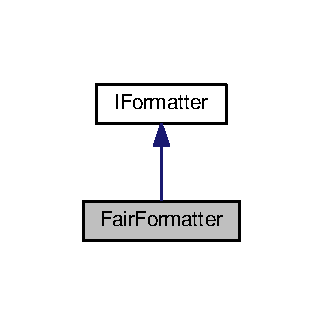
\includegraphics[width=155pt]{classFairFormatter__inherit__graph}
\end{center}
\end{figure}


Collaboration diagram for Fair\+Formatter\+:\nopagebreak
\begin{figure}[H]
\begin{center}
\leavevmode
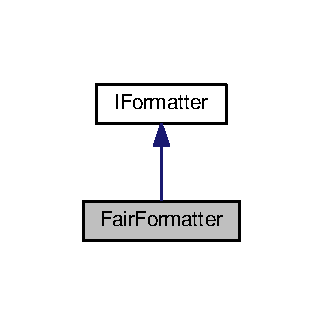
\includegraphics[width=155pt]{classFairFormatter__coll__graph}
\end{center}
\end{figure}
\subsection*{Public Member Functions}
\begin{DoxyCompactItemize}
\item 
\hypertarget{classFairFormatter_aac192190ad2cd8e5e4502244a018349c}{}virtual Return\+Value\+E {\bfseries format\+\_\+table} (\hyperlink{classTable}{Table} \&table, char \&vert\+\_\+sep, char \&horz\+\_\+sep, char \&joint\+\_\+sep)\label{classFairFormatter_aac192190ad2cd8e5e4502244a018349c}

\end{DoxyCompactItemize}


The documentation for this class was generated from the following files\+:\begin{DoxyCompactItemize}
\item 
fair\+\_\+formatter.\+h\item 
fair\+\_\+formatter.\+cpp\end{DoxyCompactItemize}

\hypertarget{classIFormatter}{}\section{I\+Formatter Class Reference}
\label{classIFormatter}\index{I\+Formatter@{I\+Formatter}}


Inheritance diagram for I\+Formatter\+:\nopagebreak
\begin{figure}[H]
\begin{center}
\leavevmode
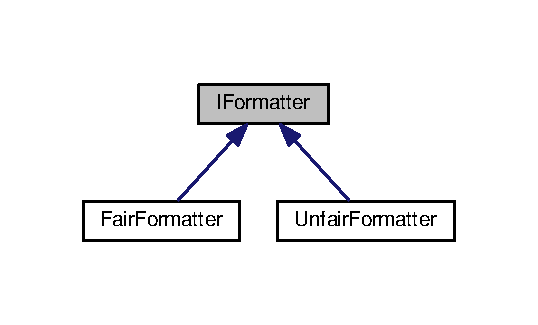
\includegraphics[width=258pt]{classIFormatter__inherit__graph}
\end{center}
\end{figure}
\subsection*{Public Member Functions}
\begin{DoxyCompactItemize}
\item 
\hypertarget{classIFormatter_ad648db87f6e7574b5301d9c904213cc3}{}virtual Return\+Value\+E {\bfseries format\+\_\+table} (\hyperlink{classTable}{Table} \&table, char \&vert\+\_\+sep, char \&horz\+\_\+sep, char \&joint\+\_\+sep)=0\label{classIFormatter_ad648db87f6e7574b5301d9c904213cc3}

\item 
\hypertarget{classIFormatter_a30bf2c73a16c03ad4157999f83cdabda}{}virtual Return\+Value\+E {\bfseries print\+\_\+border} (\hyperlink{classTable}{Table} \&table, char horz\+\_\+sep, char joint\+\_\+sep)\label{classIFormatter_a30bf2c73a16c03ad4157999f83cdabda}

\item 
\hypertarget{classIFormatter_acb93ff067902af675482b9dc02fdbb05}{}virtual Return\+Value\+E {\bfseries print\+\_\+elements} (\hyperlink{classTable}{Table} \&table, unsigned int row, char vert\+\_\+sep)\label{classIFormatter_acb93ff067902af675482b9dc02fdbb05}

\end{DoxyCompactItemize}


The documentation for this class was generated from the following files\+:\begin{DoxyCompactItemize}
\item 
iformatter.\+h\item 
iformatter.\+cpp\end{DoxyCompactItemize}

\hypertarget{classParser}{}\section{Parser Class Reference}
\label{classParser}\index{Parser@{Parser}}


\hyperlink{classParser}{Parser}\+: This class parses a given file using a user-\/defined separator as a demiliter and generates a 2\+D string vector.  




{\ttfamily \#include $<$parser.\+h$>$}

\subsection*{Static Public Member Functions}
\begin{DoxyCompactItemize}
\item 
\hypertarget{classParser_a7234c87779b6d22505f6f8849fc31ba1}{}static Return\+Value\+E \hyperlink{classParser_a7234c87779b6d22505f6f8849fc31ba1}{parse\+\_\+file} (const string filename, const char separator, Table\+Vector \&parsed\+\_\+file)\label{classParser_a7234c87779b6d22505f6f8849fc31ba1}

\begin{DoxyCompactList}\small\item\em Generates a 2\+D string vector from the input file using a user-\/defined separator. \end{DoxyCompactList}\item 
\hypertarget{classParser_aad02668636aaa522d63cdcd20035a3f9}{}static Return\+Value\+E \hyperlink{classParser_aad02668636aaa522d63cdcd20035a3f9}{parse\+\_\+line} (const string input\+\_\+line, const char separator, Row\+Vector \&parsed\+\_\+line)\label{classParser_aad02668636aaa522d63cdcd20035a3f9}

\begin{DoxyCompactList}\small\item\em Generates a string vector from a line in input file using a user-\/define seperator. \end{DoxyCompactList}\end{DoxyCompactItemize}


\subsection{Detailed Description}
\hyperlink{classParser}{Parser}\+: This class parses a given file using a user-\/defined separator as a demiliter and generates a 2\+D string vector. 

The documentation for this class was generated from the following files\+:\begin{DoxyCompactItemize}
\item 
parser.\+h\item 
parser.\+cpp\end{DoxyCompactItemize}

\hypertarget{classTable}{}\section{Table Class Reference}
\label{classTable}\index{Table@{Table}}


Maintains the data structures required to generated a formatted table. It\textquotesingle{}s main function is to store the width of the columns.  




{\ttfamily \#include $<$table.\+h$>$}

\subsection*{Public Member Functions}
\begin{DoxyCompactItemize}
\item 
\hypertarget{classTable_abb5d65b9ea5f69211ac4233cc09a5520}{}{\bfseries Table} (Table\+Vector \&in\+\_\+table, \hyperlink{classIFormatter}{I\+Formatter} $\ast$\&f, char v\+\_\+sep= \textquotesingle{}$\vert$\textquotesingle{}, char h\+\_\+sep= \textquotesingle{}-\/\textquotesingle{}, char j\+\_\+sep= \textquotesingle{}+\textquotesingle{})\label{classTable_abb5d65b9ea5f69211ac4233cc09a5520}

\item 
\hypertarget{classTable_a6364ca2696a5c3d2957c21ddf5ceb57d}{}\hyperlink{classTable}{Table} {\bfseries operator=} (const \hyperlink{classTable}{Table} \&)\label{classTable_a6364ca2696a5c3d2957c21ddf5ceb57d}

\item 
\hypertarget{classTable_a8f90634e34d019046c9b746d1717c2b2}{}int \hyperlink{classTable_a8f90634e34d019046c9b746d1717c2b2}{size} ()\label{classTable_a8f90634e34d019046c9b746d1717c2b2}

\begin{DoxyCompactList}\small\item\em Returns the size of the \hyperlink{classTable}{Table}. \end{DoxyCompactList}\item 
\hypertarget{classTable_a2052e3562592455c8d8a1f9239467d30}{}Return\+Value\+E \hyperlink{classTable_a2052e3562592455c8d8a1f9239467d30}{columns} ()\label{classTable_a2052e3562592455c8d8a1f9239467d30}

\begin{DoxyCompactList}\small\item\em Calculates the max number of columns in the table. \end{DoxyCompactList}\item 
\hypertarget{classTable_a07ee370d2224be5780d5a2d31b729ed9}{}Return\+Value\+E \hyperlink{classTable_a07ee370d2224be5780d5a2d31b729ed9}{column\+\_\+widths} ()\label{classTable_a07ee370d2224be5780d5a2d31b729ed9}

\begin{DoxyCompactList}\small\item\em Generates column widths and stores in a vector. \end{DoxyCompactList}\item 
\hypertarget{classTable_a570d9a50965036c614d2328dde1dfe8e}{}Return\+Value\+E \hyperlink{classTable_a570d9a50965036c614d2328dde1dfe8e}{get\+\_\+columns} (unsigned int \&col)\label{classTable_a570d9a50965036c614d2328dde1dfe8e}

\begin{DoxyCompactList}\small\item\em Returns the number of columns in the table. \end{DoxyCompactList}\item 
\hypertarget{classTable_aecd59c6e6420a2833de9cd6dc3df5be8}{}Return\+Value\+E \hyperlink{classTable_aecd59c6e6420a2833de9cd6dc3df5be8}{get\+\_\+rows} (unsigned int \&row)\label{classTable_aecd59c6e6420a2833de9cd6dc3df5be8}

\begin{DoxyCompactList}\small\item\em Returns the number of rows in the table. \end{DoxyCompactList}\item 
\hypertarget{classTable_ad3cb46364300d9f97655e6d628333c43}{}Return\+Value\+E \hyperlink{classTable_ad3cb46364300d9f97655e6d628333c43}{get\+\_\+column\+\_\+width} (const unsigned int \&col, unsigned int \&col\+\_\+width)\label{classTable_ad3cb46364300d9f97655e6d628333c43}

\begin{DoxyCompactList}\small\item\em Returns width of a specific column. \end{DoxyCompactList}\item 
\hypertarget{classTable_a4b480f91c567559b09ffcca9b41b38cd}{}Return\+Value\+E \hyperlink{classTable_a4b480f91c567559b09ffcca9b41b38cd}{set\+\_\+formatter} (\hyperlink{classIFormatter}{I\+Formatter} $\ast$\&f)\label{classTable_a4b480f91c567559b09ffcca9b41b38cd}

\begin{DoxyCompactList}\small\item\em Sets the formatter to be used. \end{DoxyCompactList}\item 
\hypertarget{classTable_ad0da3c76a9efeded5081ac73e81fb282}{}Return\+Value\+E \hyperlink{classTable_ad0da3c76a9efeded5081ac73e81fb282}{get\+\_\+element} (unsigned int \&row, unsigned int \&col, string \&element)\label{classTable_ad0da3c76a9efeded5081ac73e81fb282}

\begin{DoxyCompactList}\small\item\em Returns the element at the specified position. \end{DoxyCompactList}\item 
\hypertarget{classTable_a6cd0418b59cf0e6e1552587e3d84a776}{}Return\+Value\+E \hyperlink{classTable_a6cd0418b59cf0e6e1552587e3d84a776}{print\+\_\+table} ()\label{classTable_a6cd0418b59cf0e6e1552587e3d84a776}

\begin{DoxyCompactList}\small\item\em Prints the table using the Formatter specified. \end{DoxyCompactList}\end{DoxyCompactItemize}


\subsection{Detailed Description}
Maintains the data structures required to generated a formatted table. It\textquotesingle{}s main function is to store the width of the columns. 

The documentation for this class was generated from the following files\+:\begin{DoxyCompactItemize}
\item 
table.\+h\item 
table.\+cpp\end{DoxyCompactItemize}

\hypertarget{classUnfairFormatter}{}\section{Unfair\+Formatter Class Reference}
\label{classUnfairFormatter}\index{Unfair\+Formatter@{Unfair\+Formatter}}


Inheritance diagram for Unfair\+Formatter\+:\nopagebreak
\begin{figure}[H]
\begin{center}
\leavevmode
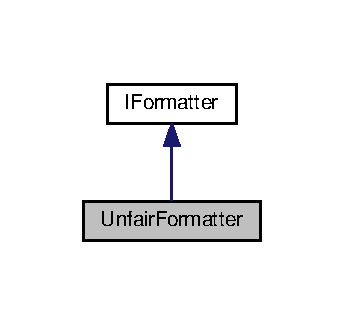
\includegraphics[width=165pt]{classUnfairFormatter__inherit__graph}
\end{center}
\end{figure}


Collaboration diagram for Unfair\+Formatter\+:\nopagebreak
\begin{figure}[H]
\begin{center}
\leavevmode
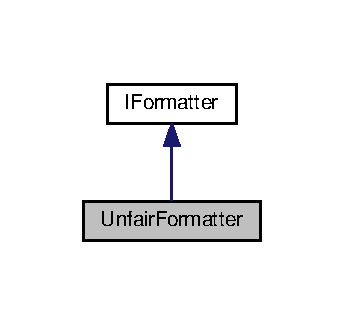
\includegraphics[width=165pt]{classUnfairFormatter__coll__graph}
\end{center}
\end{figure}
\subsection*{Public Member Functions}
\begin{DoxyCompactItemize}
\item 
\hypertarget{classUnfairFormatter_a3dc95e05cfcc097fbfc9c2d195a69453}{}virtual Return\+Value\+E {\bfseries format\+\_\+table} (\hyperlink{classTable}{Table} \&table, char \&vert\+\_\+sep, char \&horz\+\_\+sep, char \&joint\+\_\+sep)\label{classUnfairFormatter_a3dc95e05cfcc097fbfc9c2d195a69453}

\end{DoxyCompactItemize}


The documentation for this class was generated from the following files\+:\begin{DoxyCompactItemize}
\item 
unfair\+\_\+formatter.\+h\item 
unfair\+\_\+formatter.\+cpp\end{DoxyCompactItemize}

%--- End generated contents ---

% Index
\backmatter
\newpage
\phantomsection
\clearemptydoublepage
\addcontentsline{toc}{chapter}{Index}
\printindex

\end{document}
